\documentclass{beamer}
\usepackage[T1]{fontenc}

%\documentclass[aspectratio=169]{beamer}
%\usetheme{Madrid} % My favorite!
%\usetheme{Boadilla} % Pretty neat, soft color.
%\usetheme{default}
%\usetheme{Warsaw}
%\usetheme{Bergen} % This template has nagivation on the left
\usetheme{Frankfurt} % Similar to the default 
%with an extra region at the top.
\usecolortheme{seahorse} % Simple and clean template
%\usetheme{Darmstadt} % not so good
% Uncomment the following line if you want %
% page numbers and using Warsaw theme%
% \setbeamertemplate{footline}[page number]
%\setbeamercovered{transparent}
\setbeamercovered{invisible}
\setbeamersize{text margin right=3.5mm, text margin left=7.5mm}  % text margin
% To remove the navigation symbols from 
% the bottom of slides%
%
\usepackage{graphicx}

\usepackage[
backend=biber,
natbib=true,
style=numeric,
sorting=none]{biblatex}

\addbibresource{PDW-15.bib}
\usepackage{tikz}
\usepackage{calc}


\usepackage{amsmath,amsthm, amssymb, latexsym}
\usepackage{booktabs}
\usepackage[caption=false,font=footnotesize]{subfig}
\usepackage[english]{babel}
\addto\captionsenglish{\renewcommand{\figurename}{Fig.}}

\def\checkmark{\tikz\fill[scale=0.4](0,.35) -- (.25,0) -- (1,.7) -- (.25,.15) -- cycle;} 
\def\scalecheck{\resizebox{\widthof{\checkmark}*\ratio{\widthof{x}}{\widthof{\normalsize x}}}{!}{\checkmark}}
%that's defined it - now for a test

\graphicspath{{../../Figures/}{../posters/PDW-15/figures/},{./img/}}
\DeclareGraphicsExtensions{.pdf,.png,.jpg}
%\usepackage{bm}         % For typesetting bold math (not \mathbold)
%\logo{\includegraphics[height=0.6cm]{yourlogo.eps}}
%
\title[Trust in Collaborative Marine Networks]{An Investigation into Physical and Communications Trust Frameworks \\
	for Collaborative Teams of Autonomous Underwater Vehicles}

\author{Andrew Bolster}
\institute[UoL]
{
University of Liverpool \\
\medskip
{\emph{andrew.bolster@liv.ac.uk}}\\
\vspace{0.3in}

\includegraphics[width=0.5\textwidth]{img/livuni}%
}
\date{July 1, 2015}
% \today will show current date. 
% Alternatively, you can specify a date.
%
\begin{document}
%

%\AtBeginSection[
%{
%\begin{frame}<beamer>{Table of Contents}
%  \tableofcontents[currentsection,currentsubsection, 
%  hideothersubsections, 
%  sectionstyle=show/shaded,
%  ]
%\end{frame}
%}]
\begin{frame}
  \titlepage
\end{frame}

\frame{\tableofcontents}

\section{Context}
\frame{
\frametitle{Research Context}
\begin{itemize}
  \item Project launched at QUB ECIT in 2011 under the DSTL/DGA Anglo French Defence Research Group PhD Programme under Profs. Alan Marshall and Jean-Guy Fontaine
  \item What lessons from the Mobile Ad Hoc Network (MANET) space can be transferred to the marine environment?
  \item Teams of 3 - 16 Autonomous Underwater Vehicles (AUVs) Mine countermeasures, Hydrography, and Patrol Capabilities (MHPC)
  \item Defence focus, assumption of highly capable enemy attempting to compromise communications / operations
  \item Primary Simulation/Analysis work done in 12/13
  \item Moved to UoL Oct 13 after 2 mth placement @ DSTL PDW Naval Systems / Information Systems departments.
  \item Communications Analysis work done in 13/14
\end{itemize}
}

\frame{
\frametitle{Research Collaborations}
\begin{itemize}
  \item DSTL
    \begin{itemize}
      \item Visits and Placements (Summer  '13) at DSTL Porton Down and Portsdown West
      \item CDE Exhibition, London, (Spring '12)
      \item PhD National Conferences, Oxford, London and Paris
    \end{itemize}
  \item DGA/UPMC
    \begin{itemize}
      \item DGA Conference (Autumn, '12)
      \item Visits fo CRIIF (Autumn, '12)
    \end{itemize}
  \item NATO/CMRE
    \begin{itemize}
      \item UComms'12
      \item Visits \& Ongoing data sharing with CMRE(NURC) in La Spezzia
    \end{itemize}
  \item NPL/Plextek
    \begin{itemize}
      \item CDE Project on Precision Timing for Positioning with NPL/Plextek
    \end{itemize}
\end{itemize}
}

\section{Trust in Networks}
\subsection{What do we mean by trust?}
\frame{
\frametitle{Trust in Ad-Hoc Systems}
\begin{itemize}
  \item Particularly interested in the application of Trust in Decentralised (P2P) Autonomous Systems of Systems, Autonomous Underwater Vehicles (AUVs) for example
  \item <2->Trust:\emph{The expectation of an actor performing a certain task or range of tasks within a certain confidence or probability}
  \item<3->Full System Views of Trust
    \begin{itemize}
      \item<3->{Design Trust - that a system of systems will perform as spec'd / designed in operation}
      \item<4>{Operational Trust - the systems within a larger system will perform as designed in field \checkmark}
    \end{itemize}
\end{itemize}
}
\subsection{What are TMFs?}
\frame{
\frametitle{Trust Management Frameworks}
\begin{itemize}
  \item Provide information regarding the estimated future states and operations of nodes within networks
  \item <2->``[\ldots]collecting the information necessary to establish a trust relationship and dynamically monitoring and adjusting the existing trust relationship'' - \cite{Li2007}
  \item <3->Enables nodes to form collaborative \emph{opinions} on their cohort nodes based on
    \begin{itemize}
      \item Direct Observation of Communications Behaviour (eg Successfully Forwarded Packets)
      \item Common-Neighbour Recommendation
      \item Indirect Reputation
    \end{itemize}
\end{itemize}
}
\frame{
\frametitle{Transitivity in Trust Networks}
\begin{center}
  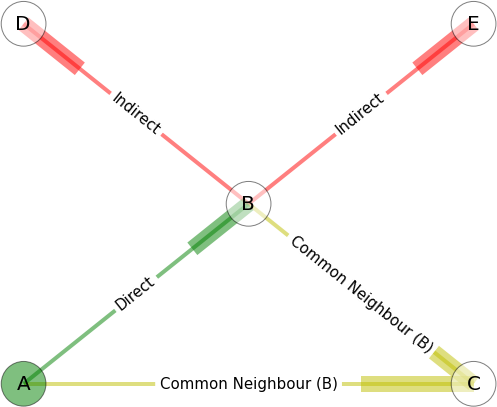
\includegraphics[height=0.6\paperheight]{img/node_relationships}
\end{center}
}

\subsection{Reasons for using Communication TMFs}
\frame{
\frametitle{TMFs in Ad Hoc Autonomous Systems}
\begin{itemize}
  \item Multiple transitive relationships can be maintained over time, providing trust resilience with dynamic network topology
  \item<2->Enable trust establishment from partial-strangers via indirect trust and direct observation
  \item<3->Enables nodes to inform internal processes for global efficiency given observed network behaviour / 'wellness', similar to those found in human social networks eg
    \begin{itemize}
      \item Update routing table based on 'safest' node chains (Phone Tree)
      \item Manoeuvre away from misbehaving nodes (Shunning)
      \item Inform as to 'trustworthiness' of forwarded information (Healthy sense of Skepticism)
      \item Historic Distrust/Trust decaying over time (Forgiveness/Relationship Decay)
    \end{itemize}
\end{itemize}
}
\frame{
\frametitle{Reason for using TMFs in MANETs}
\begin{itemize}
  \item Provide Risk Mitigation against many classical MANET attacks
    \begin{itemize}
      \item Black/Grayhole
      \item Routing Loop
      \item Selective misbehaviour / selfishness
    \end{itemize}
  \item Generally; to constrain potential malicious behaviour that can operate without detection
\end{itemize}
}

\subsection{Pre-existing Research}
\frame{
\frametitle{Trust in Autonomous Systems}
\begin{itemize}
  \item Public Key Infrastructure - Requires Centralised Control and pre-shared keys
  \item Resurrecting Duckling - Uses in-action keying with a trusted source
  \item Evidence Based Trust - Uses shared keys 
  \item Reputation Based Trust - Uses Packet forwarding success rate for prediction of future actions
    \begin{itemize}  
      \item CONFIDANT - Trust-based router implementation using packet forwarding rate
      \item Hermes - Bayesian based estimation of trust from successful interactions
      \item OTMF - Trust including transitive information from other nodes
      \item <2-> MTFM - Relationships and Multiple Metrics combined with Gray Interval assessment
    \end{itemize}
  \item \ldots and there are plenty more along the same lines
  \item Predominantly use single metrics or only communications metrics
\end{itemize}
}


\section{Multi-Metric Trust Assessment}
\subsection{Multi-Vector Trust Assessment}
\frame{
	\frametitle{The Need for Multi-Vector Trust Assessment}
	\begin{itemize}
		\item Communications not the only target for an attacker (or failure);
		\begin{itemize}
			\item Following to restricted area
			\item Masquerading
			\item Hardware Degradation
			\item Resource attack via propulsive power
		\end{itemize}
		\item Physical observation presents opportunity to further reduce the available threat surface while also discriminating between 'True' attacks and mechanical failure.
		\item Also could provide additional 'handshake' protocols for 'friendly' fleets/teams through reactionary behaviours
	\end{itemize}
	
}

\frame{
	\frametitle{Multi-Vector Trust and the Threat Surface}
	
	\begin{center}
		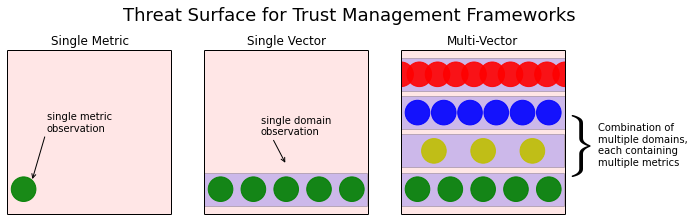
\includegraphics[width=0.9\paperwidth]{img/threat_surface_sum}
	\end{center}
	Potential attacks exist across a multi-domain threat surface
}

\subsection{Gray Trust Assessment}
\frame{
\frametitle{Multi-Parameter Trust Assessment for MANETS (MTFM)}
\begin{itemize}
  \item Application of several individual metrics for the construction of a single trust measurement
  \item For example:
    \begin{itemize}
      \item $X=\{packet\ loss, signal\ strength, data rate, delay, throughput\}$
    \end{itemize}
  \item This multi-parameter trust prevents 'smart' attackers; leveraging a known trust metric to subvert a TMF without detection
  \item Normally expressed as a vector, but can be condensed into an abstracted or weighted form for comparison \cite{Guo11}
\end{itemize}
}
\frame{
	\frametitle{Gray (MTFM) Trust Assessment}	
	\begin{align}
		\label{eq:grc}
		[\theta_{k,j}^t,\phi_{k,j}^t] & = \frac{\min_k|a_{k,j}^t - r_j^t| + \rho \max_k|a_{k,j}^t-r_j^t|}{|a_{k,j}^t-r_j^t| + \rho \max_k|a_{k,j}^t-r_j^t|},  r \in [g,b] \\
		\label{eq:metric_weighting}
		[\theta_k^t, \phi_k^t]        & = \left[\sum_{j=0}^M h_j \theta_{k,j}^t,\sum_{j=0}^M h_j \phi_{k,j}^t \right]                                                     \\
		\label{eq:trust_value}
		T_k^t                         & = ({1+{(\phi_k^t)^2}/{(\theta_k^t)^2}})^{-1}                                                                                      
	\end{align}
	where $a_{k,j}^t$ is the value of an observed metric $x_j$ for a given node $k$ at time $t$, $\rho$ is a distinguishing coefficient set to $0.5$, $g$ and $b$ are respectively the ``good'' and ``bad'' reference metric sequences from $a$, i.e. $g_j=\max_k({a_{k,j}^t})$,  $b_j=\min_k({a_{k,j}^t})$ 
	
	These metric coefficients are then accumulated \eqref{eq:metric_weighting} and combined to present a singular trust value for analysis \eqref{eq:trust_value}.
}

\frame{
\frametitle{Malicious Behaviour Discrimination}
\begin{center}
  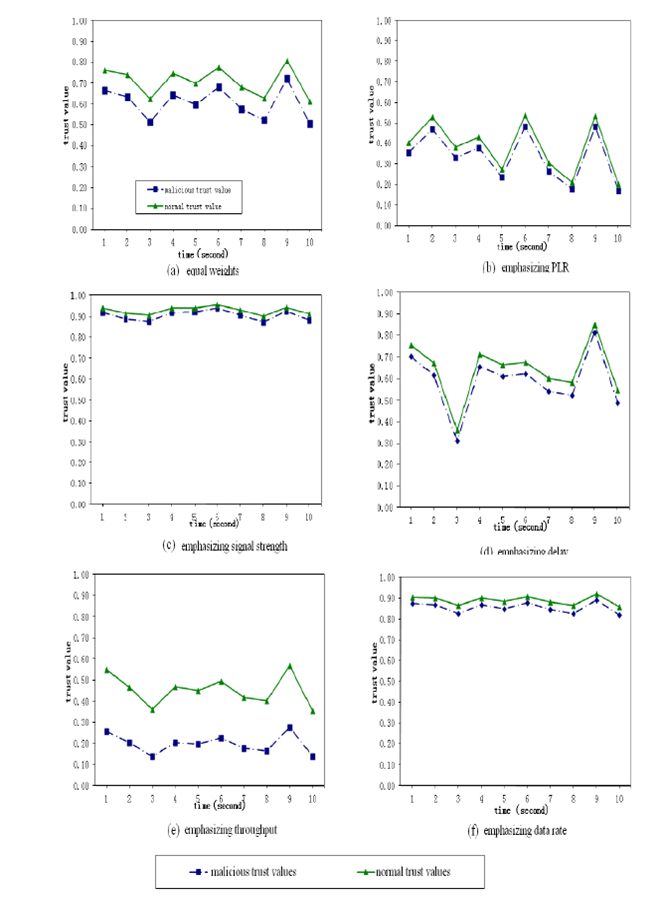
\includegraphics[height=0.8\paperheight]{img/bellas_vector_detector}
\end{center}
}



\subsection{Trust From Physical Behaviours}
\frame{
\frametitle{Agent Based Behaviour Simulator}
\begin{center}
  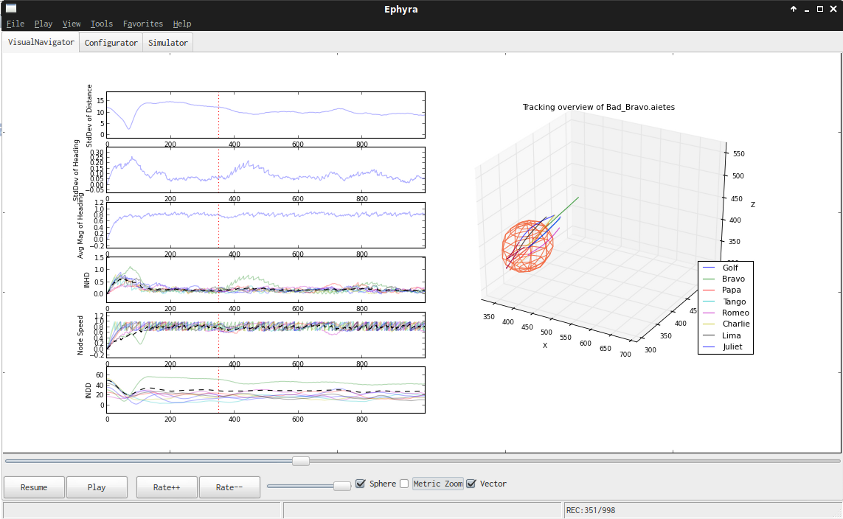
\includegraphics[width=0.9\paperwidth]{img/ephyra_vis}
\end{center}
}



\frame{
\frametitle{Operational Mission Profiles}
\begin{itemize}
  \item Flocking with Intent: MCM, Port Protection, Survey, Protection Detail, etc.
  \item<2-> Metric Selection in collaboration CMRE/DSTL
    \begin{itemize}
      \item Inter Node Heading Deviation
      \item Inter Node Distance Deviation
      \item Node Speed
    \end{itemize}
  \item <3-> Behaviour selection for testing
    \begin{itemize}
      \item Shadow
      \item Spy
      \item Sloth
      \item Stalker
      \item Scoundrel
      \item <4-> Slow Coach (non-malicious)
      \item <4-> Spin Doctor (non-malicious)
    \end{itemize}

\end{itemize}
}
\frame{
\frametitle{Raw Behavioural Metric Assessment in AUVs}
\begin{center}
  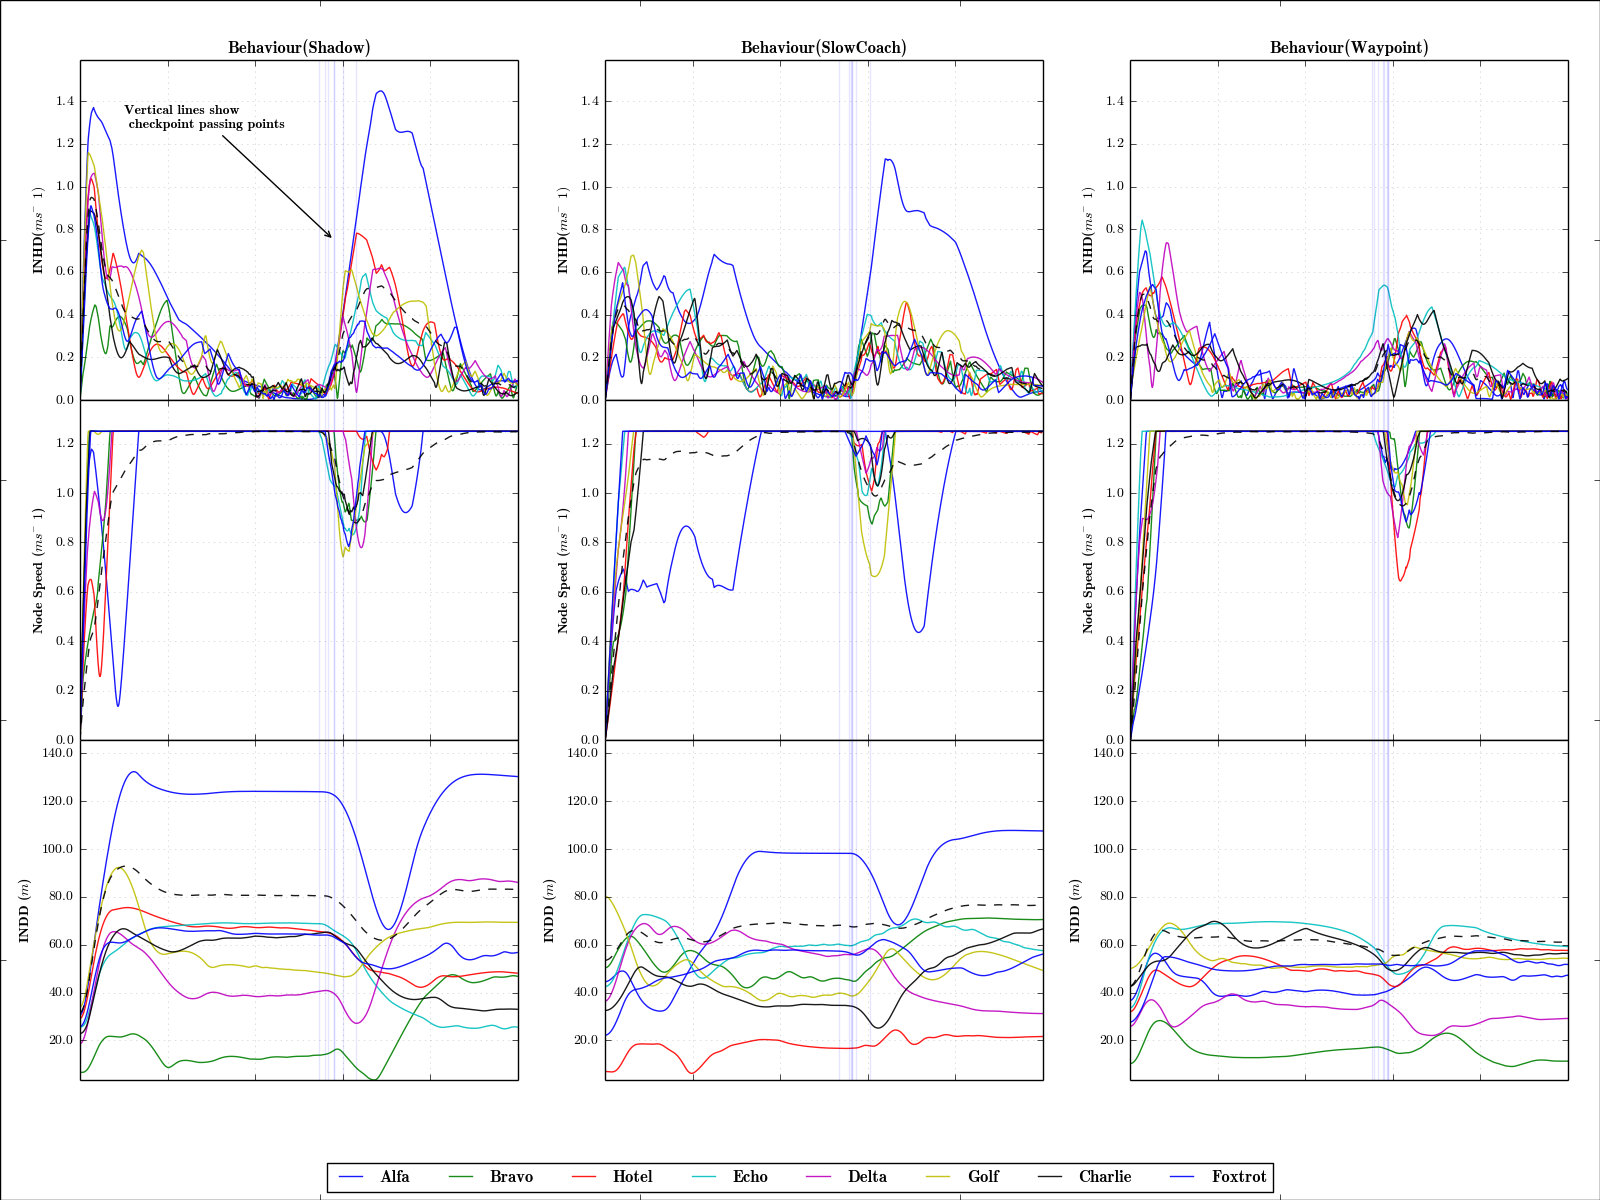
\includegraphics[height=0.8\paperheight]{img/BehaviourMetricComparison}
\end{center}
}
\frame{
\frametitle{Behavioural Trust Assessment in AUVs}
\begin{center}
  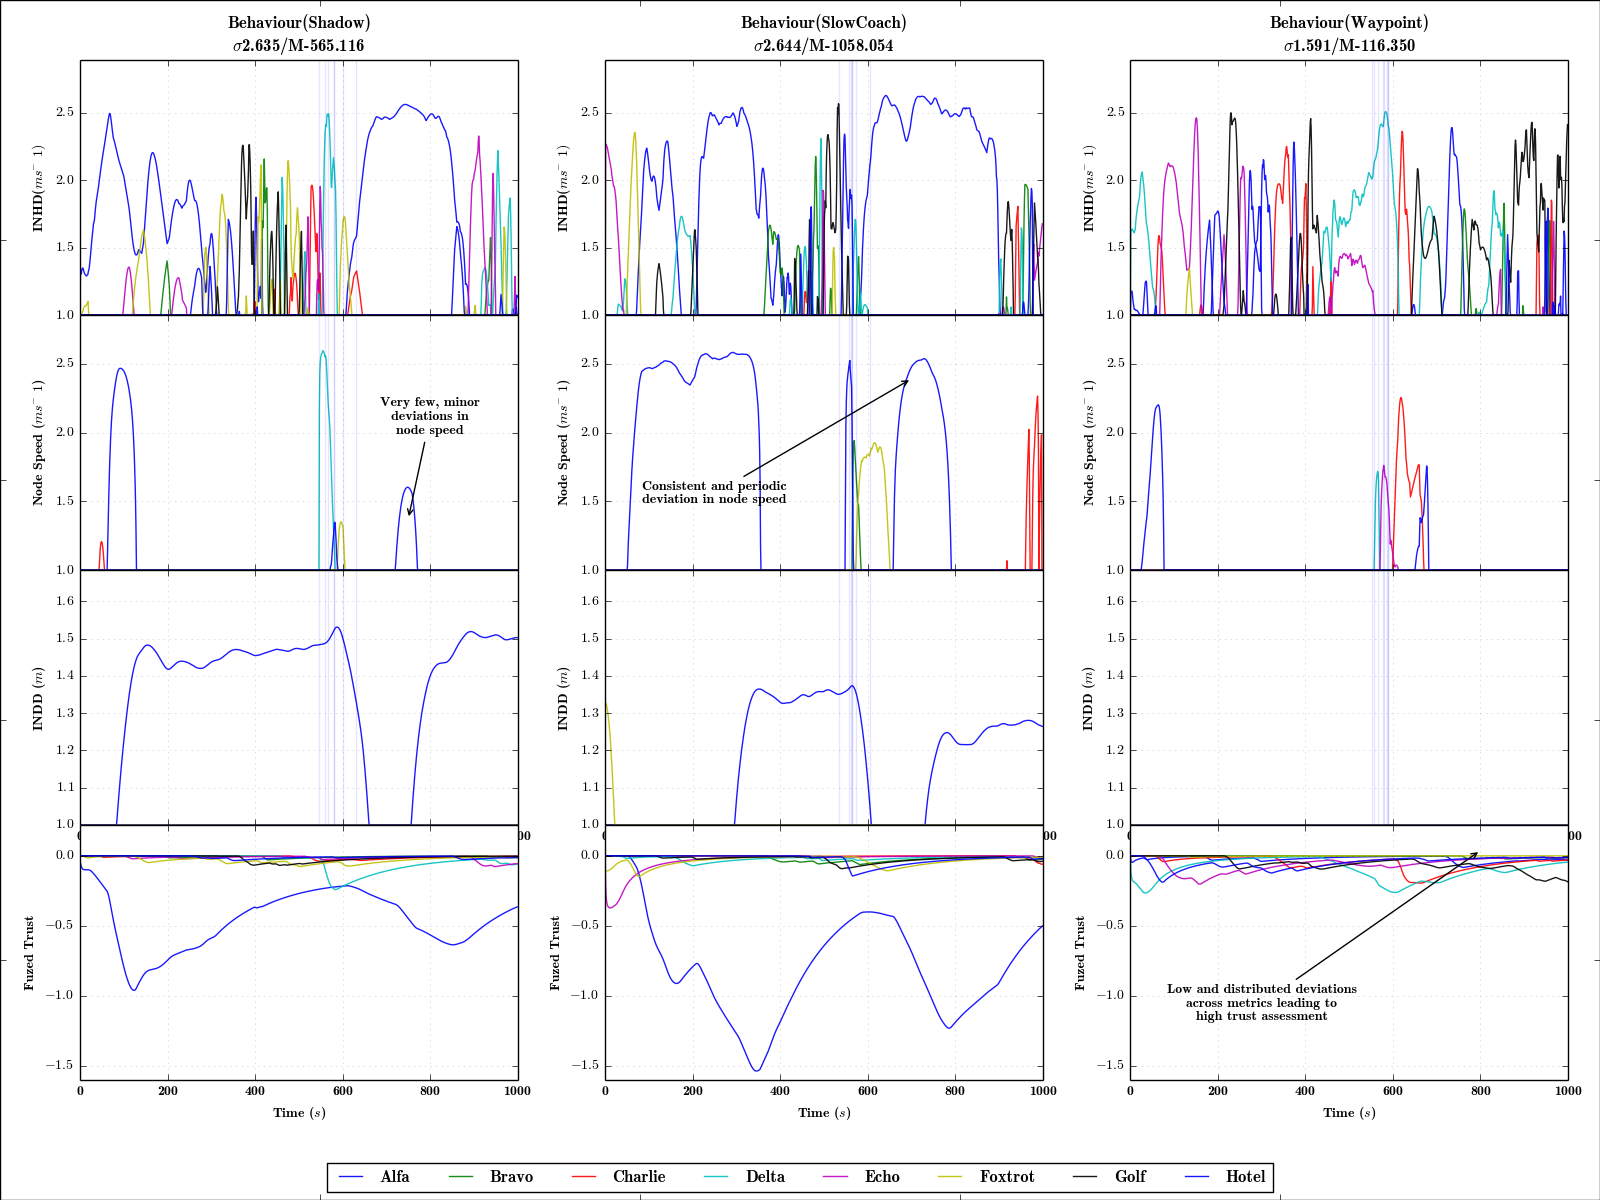
\includegraphics[height=0.8\paperheight]{img/BehaviourFusion}
\end{center}
}
\frame{
\frametitle{Behavioural Trust Assessment in AUVs}
\begin{itemize}
  \item Detection and identification based on basic weight-assessment classifier against windowed history of observations, with confidence based on a Grey Theoretic weight
  \item Currently >96\% statistical accuracy of detection and confidence, but this needs more rigorous analysis
\end{itemize}
}

\subsection{Single and Multi-Metric TMF Operation in Marine Comms}
\frame{
	\frametitle{Marine TMF Performance Assessment}
	\begin{itemize}
		\item Acoustic Network based on AUVNetSim \cite{Miquel2008} and validated against \cite{Stefanov2011}.
		\item Aim to investigate use of MTFM, against current communications TMFs (Hermes/ OTMF), which exclusively use Packet Loss Rate (PLR) as their assessment metric.  
	\end{itemize}

	Two Communications Misbehaviours were created: 
	\begin{itemize}
		\item \textbf{Malicious Power Control}(MPC) where a malicious node ($n_1$) inflates it's power to all nodes except a target node ($n_0$) making it appear selfish
		\item \textbf{Selfish Target Selection}(STS) where $n_1$ preferentially communicates with nodes that are physically near-by, reducing its own power consumption.
	\end{itemize}

}

\frame{
	\frametitle{Marine TMF Performance Assessment}
	\begin{center}
		\begin{figure}[t]
			\subfloat[Fair Scenario]{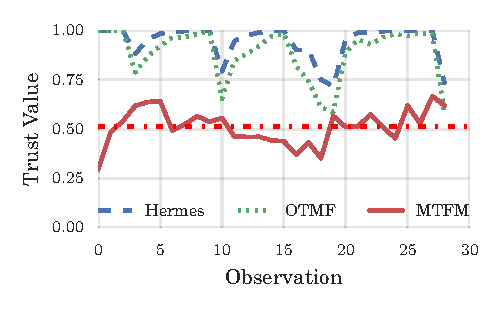
\includegraphics[width=.33\linewidth]{trust_beta_otmf_fair} \label{fig:all_mobile_fair_beta}}
			\subfloat[MPC Scenario]{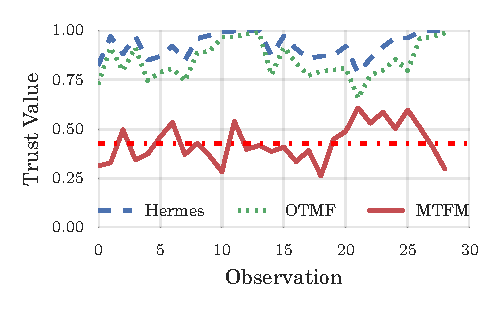
\includegraphics[width=.33\linewidth]{trust_beta_otmf_malicious} \label{fig:all_mobile_badmouthing_beta}}
			\subfloat[STS Scenario]{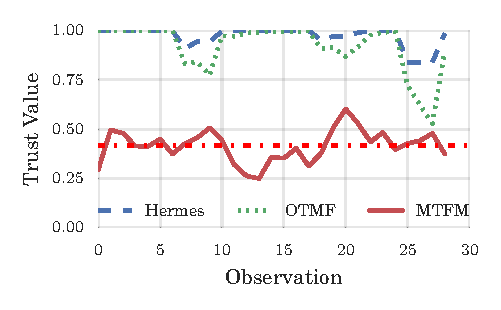
\includegraphics[width=.33\linewidth]{trust_beta_otmf_selfish} \label{fig:all_mobile_selfish_beta}}
			\caption{$T_{1,0}$ for Hermes, OTMF and MTFM assessment values for fair and malicious behaviours in the fully mobile scenario (mean of MTFM also shown)}
			\label{fig:otmf_beta_comparison}
		\end{figure}
		
		From ~\ref{fig:otmf_beta_comparison}, in the challenging underwater environment, no assessment tool is able to appreciably differentiate between behaviours (while MTFM does display a 10\% discriminating behaviour in the a-postori average assessment, shown as a red dashed line)
		
	\end{center}
	
}
\frame{
	\frametitle{Metric Emphasis and Misbehaviour detectibility: MPC}
	\begin{center}
		\begin{figure}[h]
			\subfloat[Delay]{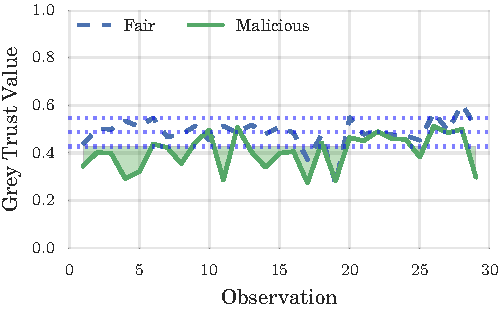
\includegraphics[width=.3\linewidth]{trust_bella_all_mobile_emph_ADelay_BadMouthingPowerControl} \label{fig:all_mobile_selfish_delay}}
			\subfloat[PLR]{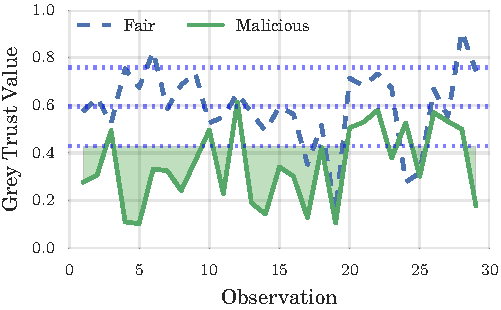
\includegraphics[width=.3\linewidth]{trust_bella_all_mobile_emph_PLR_BadMouthingPowerControl}\label{fig:all_mobile_selfish_plr}}
			\subfloat[RX Power]{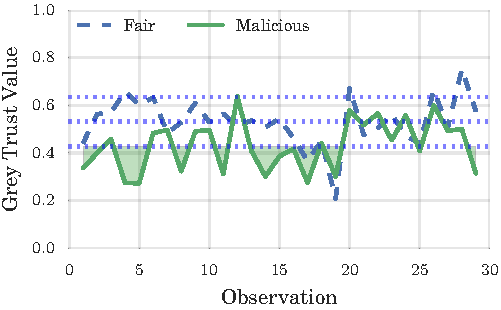
\includegraphics[width=.3\linewidth]{trust_bella_all_mobile_emph_ARXP_BadMouthingPowerControl} \label{fig:all_mobile_selfish_rxp}}
			\newline
			\subfloat[TX Power]{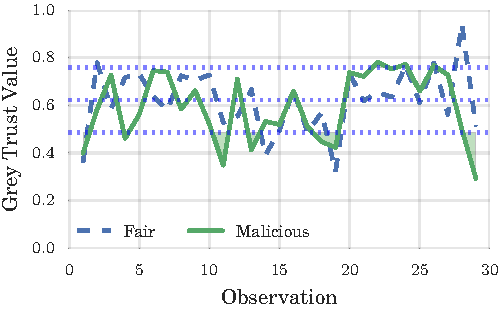
\includegraphics[width=.3\linewidth]{trust_bella_all_mobile_emph_ATXP_BadMouthingPowerControl}\label{fig:all_mobile_selfish_txp}}
			\subfloat[RX Throughput]{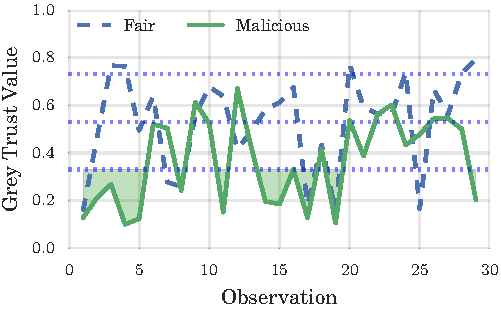
\includegraphics[width=.3\linewidth]{trust_bella_all_mobile_emph_RXThroughput_BadMouthingPowerControl} \label{fig:all_mobile_selfish_rxthroughput}}
			\subfloat[TX Throughput]{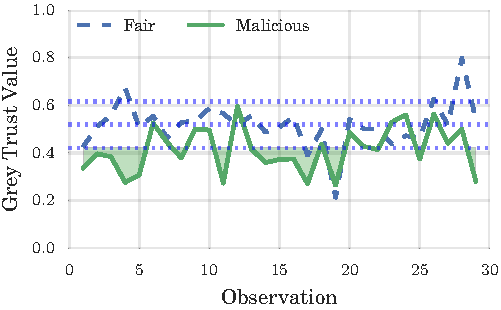
\includegraphics[width=.3\linewidth]{trust_bella_all_mobile_emph_TXThroughput_BadMouthingPowerControl} \label{fig:all_mobile_selfish_txthroughput}}
			\caption{$T_{1,MTFM}$ in the All Mobile case for the MPC behaviour, including dashed $\pm\sigma$ envelope about the fair scenario}
			\label{fig:all_mobile_selfish}
		\end{figure}
	\end{center}
	
}
\frame{
	\frametitle{Metric Emphasis and Misbehaviour detectibility: STS}
	\begin{center}
		\begin{figure}[h]
			\subfloat[Delay]{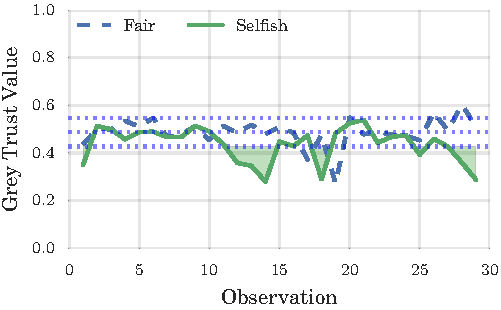
\includegraphics[width=.3\linewidth]{trust_bella_all_mobile_emph_ADelay_SelfishTargetSelection} \label{fig:all_mobile_selfish_delay}}
			\subfloat[PLR]{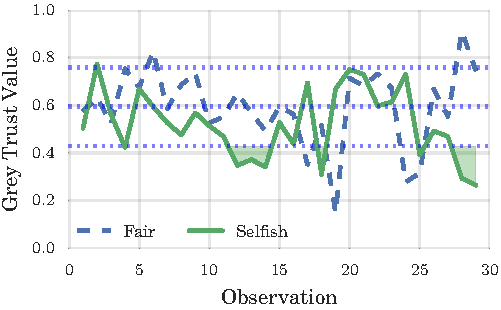
\includegraphics[width=.3\linewidth]{trust_bella_all_mobile_emph_PLR_SelfishTargetSelection}\label{fig:all_mobile_selfish_plr}}
			\subfloat[RX Power]{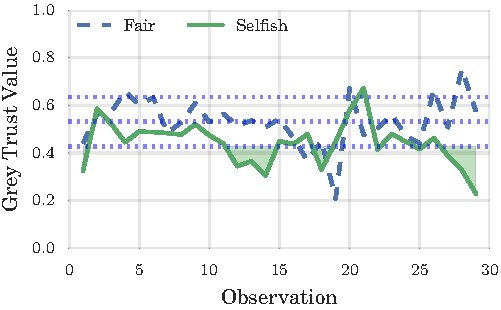
\includegraphics[width=.3\linewidth]{trust_bella_all_mobile_emph_ARXP_SelfishTargetSelection} \label{fig:all_mobile_selfish_rxp}}
			\newline
			\subfloat[TX Power]{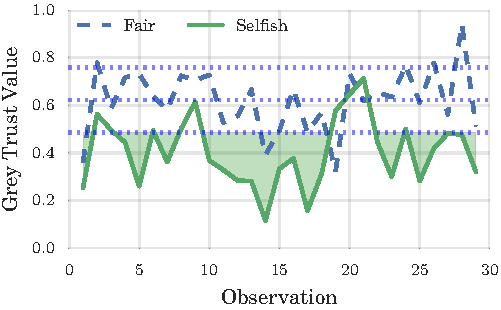
\includegraphics[width=.3\linewidth]{trust_bella_all_mobile_emph_ATXP_SelfishTargetSelection}\label{fig:all_mobile_selfish_txp}}
			\subfloat[RX Throughput]{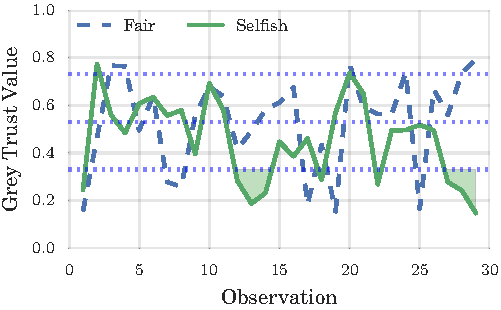
\includegraphics[width=.3\linewidth]{trust_bella_all_mobile_emph_RXThroughput_SelfishTargetSelection} \label{fig:all_mobile_selfish_rxthroughput}}
			\subfloat[TX Throughput]{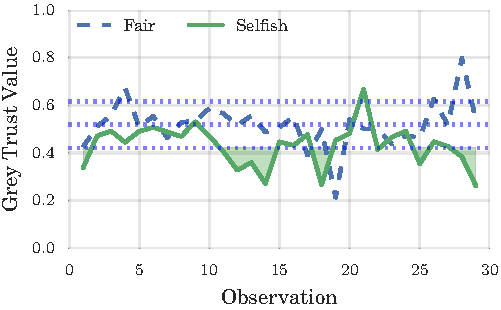
\includegraphics[width=.3\linewidth]{trust_bella_all_mobile_emph_TXThroughput_SelfishTargetSelection} \label{fig:all_mobile_selfish_txthroughput}}
			\caption{$T_{1,MTFM}$ in the All Mobile case for the STS behaviour, including dashed $\pm\sigma$ envelope about the fair scenario}
			\label{fig:all_mobile_selfish}
		\end{figure}
	\end{center}
	
}
\frame{
	\frametitle{Weight Significance Analysis for Behaviour Classification}
	Applying a Random Forest regression tree to 729 different weighting schemes for each of the three behaviours; 
	\begin{center}
		\begin{figure}
			\centering
			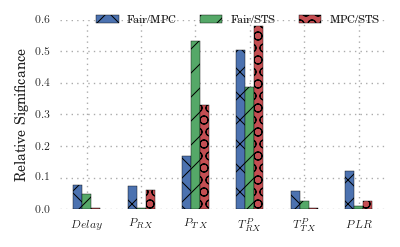
\includegraphics[width=0.65\linewidth]{MaliciousSelfishMetricFactors}
			\caption{Random Forest Factor Analysis of Malicious (MPC), Selfish (STS) and Fair behaviours compared against each-other}
			\label{fig:malselfactors}
		\end{figure}
	\end{center}
	
}
\frame{
	\frametitle{Weight Significance Analysis for Behaviour Classification}
	Applying a Random Forest regression tree to 729 different weighting schemes for each of the three behaviours; 
	\begin{center}
		\begin{table}[h]
			\caption{Correlation Coefficients between metric weights and behaviour detection targets} \label{tab:correlations}
			\begin{center}
				\begin{tabular}{lcccccc}
					\toprule
					Correlation      & Delay & $P_{RX}$ & $P_{TX}$ & $T^P_{RX}$ & $T^P_{TX}$ & PLR \\
					\midrule
					Fair / MPC       & 0.199 &  0.159   & -0.416  &  0.708   & -0.238   & -0.401\\
					Fair / STS       & 0.179 &  -0.009  &  0.724  & -0.697   & -0.145   & -0.052\\
					MPC / STS        & 0.058 &  -0.134  &  0.146  & -0.768   &  0.052   &  0.146\\
					\bottomrule
				\end{tabular}
			\end{center}
		\end{table}
	\end{center}
	
}

\frame{
	\frametitle{Remaining Work and Analysis}
	\begin{itemize}
		\item Perform Cross and Inter-Domain analysis between Comms and Behavioural Environment \emph{Preliminary results available on request}
		\item Extension of MTFM to be asynchronous and report-delay tolerant (back-propagation of delayed messages)
		
	\end{itemize}
	
}

\subsection{Challenges for Implementing Multi-vector Trust}
\frame{
\frametitle{Challenges in Multi-vector Trust}
\begin{itemize}
  \item How to define optimality in trust assessment when dealing with multiple vectors and transitive trust?
  \item Is there a quantifiable benefit to cross-domain comparison beyond single vector Trust?
  \item Is there an optimal generic cross-domain comparator?
\end{itemize}
}

\section{Outputs and Remaining Work}
\subsection{Publications}

\frame{
\frametitle{Current Publications}
\begin{itemize}
\item A Multi-Vector Trust Framework for Autonomous Systems \cite{Bolster2014}
  \begin{itemize}
  \item Symposium paper to the Association for the Advancement of Artificial Intelligence on the current state of work, presenting our progress towards multi-vector trust
  \end{itemize}


\item \textsc{Analysis of Trust Interfaces in Autonomous and Semi-Autonomous Collaborative MHPC Operations \cite{Bolster2014a}}
  \begin{itemize}
  \item Part of a Five-Eyes defence strategy programme (TTCP) for assuring C3I capabilities as part of FF2020
  \end{itemize}

\item Single and Multi-Metric Trust Management Frameworks for use in Underwater Autonomous Networks
\begin{itemize}
	\item Submitted to TrustCom15: Decision Pending
\end{itemize}

\item Multi-Domain Trust Management Framework for Underwater Autonomous Networks
\begin{itemize}
	\item Awaiting submission to InfoCom15
\end{itemize}

\end{itemize}
}
\subsection{Thesis Plan}
\frame[allowframebreaks]{
\frametitle{Thesis Plan}
\begin{enumerate} 
	\item Background Information on Trust and its applications to MANETs
	\begin{itemize}
		\item Discussion on abstract analysis of trust networks
		\item Discussion on the threat surface of Mobile Ad Hoc Networks and how that has been protected so far
		\item Introduction to Trust Management Frameworks and their benefits
	\end{itemize}
	\item Background Information on Maritime Uses of Autonomous Systems
	\begin{itemize}
		\item Discussion of current and future approaches to areas where autonomous systems can be used mainly focused on Mine counter measures, Hydrography and Patrol Capabilities (MHPC)
		\item Discussion of the contextual human factors around integrating autonomous systems into existing human-based solutions.
		\item Predominantly following on from work already accomplished under ``Analysis of Trust Interfaces in Autonomous and Semi-Autonomous Collaborative MHPC Operations'', including development of representative malicious and abnormal behaviours
	\end{itemize}
	\framebreak
	\item Strategies for Multi-Domain Trust Assessment
	\begin{itemize}
		\item Analytical establishment of Multi-Domain Trust, from an information theoretic standpoint.
	\end{itemize}
	\item Modelling and Analysis of Collaborative Node Kinematic Behaviours in Underwater Acoustic MANETS
	\begin{itemize}
		\item Touching on the development of the simulation platform but focused on the mobility and assessment of mobility between nodes, including identification of suitable motive metrics and analyses of these motions to establish intent or abnormality
		\item Passing mention of work done in Drift analysis with NPL/Plextek as supporting evidence
	\end{itemize}
	\item Comparative Analysis of Multi-Domain Trust Assessment in Collaborative Mobile Networks
	\item Investigation into the relative performance characteristics of multi-domain combination strategies in an exemplary context (AUV teams) against existing single and multi metric TMFs
\end{enumerate}
}


%
\begin{frame}[t,allowframebreaks]
  \frametitle{References}
  \printbibliography[title=References]% [nottype=video]}
\end{frame}

\begin{frame}
  \centerline{The End}
\end{frame}
% End of slides
\end{document} 


